\documentclass[10pt,a4paper]{article}
\usepackage[utf8]{inputenc} % para poder usar tildes en archivos UTF-8
\usepackage[spanish]{babel} % para que comandos como \today den el resultado en castellano
\usepackage{a4wide} % márgenes un poco más anchos que lo usual
\usepackage[conEntregas]{Sty/caratula}
\usepackage{Sty/mathtools}
\usepackage{Sty/float}
\usepackage[pdftex]{graphicx}
\usepackage{caption}
\usepackage{subcaption}
\usepackage[ruled,vlined,linesnumbered]{Sty/algorithm2e}
%Esto de abajo es para encabezado y pie de pagina
\usepackage{Sty/lastpage}
\usepackage{fancyhdr}
\usepackage{amsfonts}
\usepackage{wrapfig}
\usepackage{amsmath}
\usepackage{listings}
\usepackage{color}

\usepackage[simplified]{Sty/pgf-umlcd}

\pagestyle{fancy}


\cfoot{\thepage /\pageref{LastPage} }


\begin{document}

\fecha{\today}
\materia{Ingeniería de Software I}
\titulo{Trabajo Práctico I}

\integrante{}{}{}
\integrante{}{}{}
\integrante{}{}{}
\integrante{}{}{}
\integrante{}{}{}

\maketitle
\newpage
\tableofcontents

\newpage
\section{User Stories}
\section{User Stories}

\begin{enumerate}
  \item Como miembro del ministerio quiero que el sistema calcule el costo y la ganancia de todas las acciones simuladas sobre un yacimiento y las muestre al finalizar la ejecución para definir el mínimo monto para la licitación
  \item Como un ingeniero quiero que el sistema calcule la ganancia de la venta del petróleo extraído cada día por pozo para refinar la ganancia.
  \item Como un ingeniero quiero que el sistema no me permita excavar dos pozos en una misma parcela para agregarle valor al simulador
  \item Como un ingeniero quiero que el sistema recalcule la presión del pozo luego de un día de extracción de producto en el yacimiento para agregarle realidad al simulador
  \item Como un ingeniero quiero indicar al sistema la creación de una planta separadora para GASTO de separar el producto en petróleo, gas y agua
  \item Como un ingeniero quiero indicarle al sistema la creación de un tanque de almacenamiento para reflejar el almacenamieto de agua o gas
  \item Como un ingeniero quiero que el sistema no permita extraer de los pozos conectados a una planta más producto del que la planta puede procesar para agregarle realidad al sistema, ya que esto no puede suceder
  \item Como un ingeniero quiero que el sistema no permita procesar más producto si su porcentaje de agua o gas supera lo que se puede almacenar en los tanques para agregar realidad al sistema, ya que esto no puede suceder
  \item Como un ingeniero quiero indicarle al sistema que procese la venta de gas almacenado en los tanques para poder reflejar el aumento de almacenamiento
  \item Como un ingeniero quiero que el sistema considere la ganancia obtenida de la venta de gas almacenada en tanques para REFLEJAR la ganancia de dinero
  \item Como un ingeniero quiero poder indicarle al sistema cuál es el valor crítico de presión de los pozos que indica cuando no se debe extraer mas producto para ALGO SIMILAR AL VALOR CRITICO
  \item Como un ingeniero quiero que el sistema permita la reinyección en los pozos con agua y/o gas almacenados en los tanques para considerar el cambio de composición del producto en el yacimiento en la realidad
  \item Como un ingeniero quiero que el sistema permita la reinyección en los pozos del agua comprada para considerar el cambio de composición del producto en el yacimiento en la realidad
  \item Como un ingeniero quiero que el sistema recalcule la presión del pozo luego de la reinyección del mismo para tener en cuenta el aumento de presión utilizado en la realidad y extender la vida útil del yacimiento
  \item Como un ingeniero quiero poder indicarle al sistema cuál es la máxima cantidad que se puede reinyectar por día para evitar superar la capacidad de reinyección del pozo existente en la realidad
  \item Como un ingeniero quiero que el sistema no permita la extracción de ningún pozo durante el mismo día de una reinyección para tener un cálculo de presión mas preciso
  \item Como un ingeniero quiero poder indicarle al sistema cuál es el valor crítico (porcentaje de petróleo) que indica cuando un yacimiento llega a su fin operativo para KASJFD (redondear ganancia y despreciar muchos días de poca ganancia)
  \item Como miembro del ministerio quiero poder consultar el log de acciones simuladas sobre un yacimiento para justificar el monto de la licitación
  \item Como un ingeniero quiero indicarle al simulador que considere la creación de un pozo nuevo para poder tener un balance final mas realista
  \item Como un ingeniero quiero indicarle al simulador que considere la creación de un pozo nuevo para poder tener un balance final mas realista
  \item Como un ingeniero quiero indicarle al simulador que considere la creación de una cantidad de pozos en las parcelas con menor profundidad al yacimiento para reflejar una posible estrategia del equipo de ingeniería
  \item Como un ingeniero quiero indicarle al simulador que considere la creación de una cantidad de pozos en las parcelas cuya composición ofrezca menor resistencia a la perforación para reflejar una posible estrategia del equipo de ingeniería
  \item Como un ingeniero quiero indicarle al simulador que considere la creación de una cantidad de pozos en las parcelas con mayor presión inicial para reflejar una posible estrategia del equipo de ingeniería
  \item Como un ingeniero quiero indicarle al sistema en qué momento inicia la excavación de un pozo para LOS TIEMPOS Y LOGS SEAN MAS REALISTAS
  \item Como un ingeniero quiero poder indicarle al sistema el alquiler de un RIG para ser utilizado en la excavación de un cierto pozo para tener en cuenta el costo de la excavación de un pozo
  \item Como un ingeniero quiero poder indicarle al sistema la cantidad máxima de RIGS que pueden utilizarse simultáneamente para mejorar la estimación de costos de exavación.
  \item Como un ingeniero quiero poder indicarle al sistema que realize la excavación de los pozos utilizando la máxima cantidad posible de RIGS en simultaneo para reflejar una estrategia muy utilizada por el equipo de ingeniería.
  \item Como un ingeniero quiero poder indicar en qué momento se realiza la construcción de las plantas separadoras y/o los tanques de almacenamiento para LOS TIEMPOS Y LOGS SEAN MAS REALISTAS
  \item Como un ingeniero quiero determinarle al sistema la cantidad de pozos que se utilizan por día para extraer producto para contemplar en el simulador las decisiones que se toman en la realidad (?)
  \item Como un ingeniero quiero indircarle al simulador que al momento de extraer producto de los pozos seleccione los que tengan mayor presión para reflejar una posible estrategia del equipo de ingeniería.
  \item Como un ingeniero quiero indicarle al sistema que cuando se llegue a un nivel de presión determinado en un pozo se reinyecte el agua y gas almacenado en los tanques hasta llegar a un nivel especificado para considerar una estrategia del equipo de ingeniería
\end{enumerate}


\newpage
\section{Diseño OO}
\section{Diseño OO}

\subsection{Introducción}


\subsection{Explicación general del diseño}
\par El modelo presentado se basa en un sistema de simulación que es configurado con los siguientes subsistemas:
\begin{itemize}
  \item \textbf{Sistema de construcción}: es el encargado de crear y almacenar los planes de construcción de pozos de extracción, plantas procesadoras y tanques de almacenamiento. También almacena los catálogos de plantas procesadoras y tanques de almacenamiento y gestiona las conexiones entre pozos de excavación, tanques de almacenamiento y plantas procesadoras.
  \item \textbf{Sistema de ejecución de criterios}: se encarga de llevar a cabo la ejecución de cada criterio del sistema.
  \item \textbf{Sistema de gestión de excavadoras}: posee el catálogo de excavadoras y gestiona su alquiler. También almacena el estado de las excavadoras alquiladas.
  \item \textbf{Sistema de gestión de parcelas}: Es quien conoce al yacimiento y administra las parcelas utilizadas y libres.
  \item \textbf{Sistema de extracción y reinyección}: Es quien se encarga de crear los eventos de extracción y reinyección sobre los pozos y almacenarlos.
\end{itemize}

\begin{tikzpicture}
  \node[shape=circle,draw=black] (unSimulador) at (0,0) {\shortstack{\textbf{unSimulador}:\\SistemaDe\\Simulacion}};
  \node[shape=circle,draw=black] (unSistemaDeConstruccion) at (-6,-2) {\shortstack{\textbf{unSistemaDe}\\\textbf{Construcción}:\\SistemaDe\\Construccion}};
  \node[shape=circle,draw=black] (unSistemaDeEjecucionDeCriterios) at (-4,-5) {\shortstack{\textbf{unSistemaDe}\\\textbf{EjecucionDe}\\\textbf{Criterios}:\\SistemaDe\\EjecucionDe\\Criterios}};
  \node[shape=circle,draw=black] (unSistemaDeGestionDeExcavadoras) at (0,-6) {\shortstack{\textbf{unSistemaDe}\\\textbf{GestionDe}\\\textbf{Excavadoras}:\\SistemaDe\\GestionDe\\Excavadoras}};
  \node[shape=circle,draw=black] (unSistemaDeGestionDeParcelas) at (4,-5) {\shortstack{\textbf{unSistemaDe}\\\textbf{GestionDe}\\\textbf{Parcelas}:\\SistemaDe\\GestionDe\\Parcelas}};
  \node[shape=circle,draw=black] (unSistemaDeExtraccion) at (6,-2) {\shortstack{\textbf{unSistemaDe}\\\textbf{ExtraccionY}\\\textbf{Reinyección}:\\SistemaDe\\ExtraccionY\\Reinyeccion}};

  \path [-] (unSimulador) edge node[left] {} (unSistemaDeConstruccion);
  \path [-] (unSimulador) edge node[left] {} (unSistemaDeEjecucionDeCriterios);
  \path [-] (unSimulador) edge node[left] {} (unSistemaDeGestionDeExcavadoras);
  \path [-] (unSimulador) edge node[left] {} (unSistemaDeGestionDeParcelas);
  \path [-] (unSimulador) edge node[left] {} (unSistemaDeExtraccion);
\end{tikzpicture}


\newpage

\subsubsection{Gestión de parcelas}
Para la gestión de parcelas decidimos hacer tres clases que auxilian al sistema de gestión de parcelas. 
\begin{itemize}
    \item Estrategia de selección de parcelas: como se comentó anteriormente esta clase se encarga de decidir que parcela va a ser seleccionada.
    \item Yacimiento: Posee el conocimiento de todo el conocimiento topológico del lugar físico donde se va a realizar la simulación.
    \item Parcela de yacimiento: Es una parte del yacimiento, en particular sólo puede ser perforada una sola vez. Posee todo el conocimiento geológico de su correspondiente lugar físico.
\end{itemize}
En el siguiente diagrama se puede ver la relaci\'on entre las clases encargadas de la gesti\'on de las parcelas:\\


\begin{figure}[ht]
    \begin{tikzpicture}
        \begin{class}{SistemaDeGestionDeParcelas}{0,-10}
            \attribute{.initializeComoParteDe: unSimulador}
            \attribute{.parcelas}
            \attribute{.usarComoFuenteDeParcelasA: unYacimiento}
            \attribute{.parcelasEnUso}
            \attribute{.parcelasLibres}
            \attribute{.utilizarParcela: unaParcela}
            \operation{.comoParteDe: unSimulador}
        \end{class}
        
        \begin{class}{EstrategiaDeSeleccionDeParcelas}{7,-9}
            \implement{SistemaDeGestionDeParcelas}
            \operation{.ejecutarEn: unSimulador}
        \end{class}
            
        \begin{class}{Yacimiento}{0,0}
            \operation{.deTamanioEnHectareas: unasHectareas volumenDeProducto: unVolumen compuestoPor: unaComposicionPorcentualDeReservorio }
            \attribute{.composicionInicial}
            \attribute{.initializeDeTamanioEnHectareas: unasHectareas volumenDeProducto: unVolumen compuestoPor: unaComposicionPorcentualDeReservorio }
            \attribute{.parcelaLibreDeTipo: unMantoGeologico presionInicial: unCantidadDePresion yDistanciaAlReservorio: unaDistanciaEnMetros}
            \attribute{.parcelasDefinidas}
            \attribute{.volumenDeProductoInicial}
        \end{class}
    
        \begin{class}{ParcelaDeYacimiento}{8,0}
            \attribute{.distanciaAlReservorio}
            \attribute{.presionInicial}
            \attribute{.resistenciaTerreno}
            \attribute{.yacimiento}
            \attribute{.printOn: aStream}
            \attribute{.initializeDeTipo: aMantoGeologico conPresionInicial: unaMedidaDePresion profunidadEnMetros: unaMedidaDeDistancia alReservorioEn: unYacimiento}
            \operation{.deTipo: unMantoGeologico conPresionInicial: unaMedidaDePresion profunidadEnMetros: unaMedidaDeDistancia alReservorioEn: unYacimiento}
        \end{class}
        \unidirectionalAssociation{Yacimiento}{parcelas}{0..*}{ParcelaDeYacimiento}
        \unidirectionalAssociation{SistemaDeGestionDeParcelas}{yacimiento}{1}{Yacimiento}
    \end{tikzpicture}
    \caption{Diagrama de clases que muestra la parte del sistema de gestión de parcelas.}
    \label{fig:dia_obj_criterios_1}
\end{figure}

\newpage


\subsubsection{Gestión de excavadoras}
\par El sistema recibe como configuración un catálogo de excavadoras que se pueden alquilar, junto con su consto por día y cantidad de días de alquiler. Esto fue modelado mediante la clase \textit{ItemDeAlquiler}. Como vemos en la figura \ref{fig:dia_cla_catalogo_1}, el sistema de gestión de excavadoras conoce una lista de items de alquiler. También conoce las excavadoras en uso y las disponibles. De esta manera, todo el que necesite utilizar excavadoras o saber sobre su situación debe consultar al sistema de gestión de excavadoras.

\begin{figure}[ht]
    \begin{tikzpicture}
        \begin{class}[text width=6cm]{SistemaDeGestionDeExcavadoras}{0,0}
            \attribute{.excavadorasDisponibles}
            \attribute{.indiceAlquilerMinimo}
            \attribute{.indicePrecio}
            \attribute{.initializeComoParteDe: unSistemaDeSimulacion }
            \operation{.comoParteDe: unSistemaDeSimulacion}
        \end{class}
        
        \begin{class}[text width=6cm]{ExcavadoraRig}{0,-7}
            \attribute{.initializePerforandoEnMetrosEnUnDia: unaMedidaEnMetros consumiendoEnLitros: unaMedidaEnLitros}
            \attribute{.profundidadPorDia}
        \end{class}
        
        
        \begin{class}{ItemDeAlquiler}{9,-1}
            \attribute{.costoPorDia}
            \attribute{.cantidadDeDias}
            \attribute{.modeloDelItem}
        \end{class}
        
        
        \unidirectionalAssociation{SistemaDeGestionDeExcavadoras}{catalogo}{0..*}{ItemDeAlquiler}
        \unidirectionalAssociation{SistemaDeGestionDeExcavadoras}{excavadorasDisponibles}{0..*}{ExcavadoraRig}
        
    \end{tikzpicture}
    \caption{Diagrama de clases que muestra al sistema de gestión de excavadoras y cómo almacena el catálogo junto con las excavadoras disponibles.}
    \label{fig:dia_cla_catalogo_1}
\end{figure}

\newpage

\subsubsection{Construcción de pozos}
Para nuestro modelo de la construcción de los pozos las dos secciones anteriores son fundamentales porque el sistema de construcción de pozos necesita conocer el terreno y con qué lo va a perforar. 
El sistema de construcción de pozos conoce al plan de construcción de pozos (encargado de conocer cuando comienza y cuando termina la construcción) y el criterio de construcción (encargado de indicar cuantos pozos hay que contruir, en qué lugar, con que excavadora y con qué estrategia).
Luego de haber presentado los dos diagramas anteriores ya podemos mostrar c\'omo diseñamos la soluci\'on para el problema de la contrucci\'on de los pozos\\

\begin{tikzpicture}
    \begin{class}{SistemaDeConstruccion}{8,-4}
        \operation{.comoParteDe: unSimulador}
        \attribute{.actualizarPlanesDePozos}
        \attribute{.comenzarConstruccionDePozoEn: unaParcela usando: unaExcavadora al: unaFecha}
    \end{class}

    \begin{class}{EstrategiaSeleccionParcelas}{10,0}
        \operation{.ejecutarEn: unSimulador}
    \end{class}
    \begin{class}{EstrategiaSeleccionExcavadoras}{10,-2}
        \attribute{.ejecutarEn: unSimulador}
    \end{class}
    \begin{class}{CriterioDeConstruccionPozo}{0,0}
        \implement{SistemaDeConstruccion}
        \attribute{.ejecutarEn: unSimulador}
        \attribute{.initializeConstruir: unaCantidad parcelasObtenidasCon: unaEstrategiaDeSeleccionDeParcelas yExcavadorasCon: unaEstrategiaDeSeleccionDeExcavadoras}
        \attribute{.siFaltanConstruirPozosEn: unSistemaDeConstruccion repetir: unBloqueDeUnArgumento}
        \attribute{.siHayDisponible: unaExcavadora realizar: unBloqueDeUnArgumento}
    \end{class}
    \begin{class}{PlanDeConstruccionDePozo}{3,-8}
        \attribute{.excavadora}
        \attribute{.fechaDeInicioDeConstruccion}
        \attribute{.fechaFinDeConstruccion}
        \attribute{.pozoDeExtraccion}
        \operation{.para: unPozoDeExtraccion cavadoCon: unaExcavadora empezandoEl: unaFecha}
    \end{class}
    \unidirectionalAssociation{CriterioDeConstruccionPozo}{}{}{EstrategiaSeleccionParcelas}
    \unidirectionalAssociation{CriterioDeConstruccionPozo}{}{}{EstrategiaSeleccionExcavadoras}
    %\unidirectionalAssociation{SistemaDeConstruccion}{}{}{SistemaDeGestionDeParcelas}
    \unidirectionalAssociation{SistemaDeConstruccion}{}{0..*}{PlanDeConstruccionDePozo}
\end{tikzpicture}


\subsubsection{Planes de construcción}

\par Como hay varios tipos de planes de construcción decidimos que lo mejor era subclasificar el plan de construcción en cada uno de los planes de construcción de cada caso, de esta manera todos estos objetos son polimórficos.

\begin{tikzpicture}
    \begin{abstractclass}{PlanDeConstruccion}{5,-9}
        \attribute{}
    \end{abstractclass}
    \begin{class}{PlanDeConstruccionDePozo}{0,-11}
        \inherit{PlanDeConstruccion}
        \attribute{.excavadora}
        \attribute{.fechaDeInicioDeConstruccion}
        \attribute{.fechaFinDeConstruccion}
        \attribute{.pozoDeExtraccion}
        \operation{.para: unPozoDeExtraccion cavadoCon: unaExcavadora empezandoEl: unaFecha}
    \end{class}
    \begin{class}{PlanDeConstruccionDePlanta}{1.5,-16}
        \inherit{PlanDeConstruccion}
        \attribute{.plantaProcesadora}
        \attribute{.fechaDeInicioDeConstruccion}
        \attribute{.fechaFinDeConstruccion}
        \operation{.para: unaPlanta empezandoEl: unaFecha yFinalizando: otraFecha}
    \end{class}
    \begin{class}{PlanDeConstruccionDeTanqueDeAgua}{8.5,-16}
       \inherit{PlanDeConstruccion}
        \attribute{.tanqueDeAgua}
        \attribute{.fechaDeInicioDeConstruccion}
        \attribute{.fechaFinDeConstruccion}
        \operation{.para: unTanque empezandoEl: unaFecha yFinalizando: otraFecha}
    \end{class}
    \begin{class}{PlanDeConstruccionDeTanqueDeGas}{10,-11}
       \inherit{PlanDeConstruccion}
        \attribute{.tanqueDeGas}
        \attribute{.fechaDeInicioDeConstruccion}
        \attribute{.fechaFinDeConstruccion}
        \operation{.para: unTanque empezandoEl: unaFecha yFinalizando: otraFecha}
    \end{class}
\end{tikzpicture}

\newpage

\subsubsection{Otras decisiones de diseño}

\par Dado que en el enunciado se mencion\'o que hab\'ia m\'as de una manera de seleccionar excavadoras, parcelas o plantas y que esa decisi\'on influ\'ia en el resultado final de la simulaci\'on vimos un intent similar al del patr\'on de diseño Strategy por lo que decidimos usar dicho patr\'on.\\


Tambi\'en ocurre algo similar con la condici\'ion de corte y la construcci\'on de las distintas edificaciones, por lo que tambi\'en usamos Strategy. \\
\vspace{1cm}

\begin{tikzpicture}
    \begin{abstractclass}{EstrategiaDeParada}{0,0}
        \attribute{.ejecutarEn: unSimulador}
    \end{abstractclass}
    \begin{class}{EstrategiaDeParadaCantDias}{0,-2}
        \inherit{EstrategiaDeParada}
        \operation{.ejecutarEn: unSimulador}
        \operation{.initializeMaxCantDiasSimulacion: unaCantidadDeDias}
    \end{class}
\end{tikzpicture}

\vspace{1cm}
En el enunciado se comenta que no se puede extraer de los pozos que est\'an en construcci\'on ni cuando la v\'alvula est\'a cerrada. Adem\'as s\'olo se puede abrir la v\'alvula de un pozo ya construido. Dada esta situaci\'on en la que hay varios estados, optamos por modelar el comportamiento de un pozo utilizando el patr\'on State.

\vspace{0.5cm}

\begin{tikzpicture}
    \begin{abstractclass}{EstadoPozoDeExtraccion}{0,5}
        \attribute{habilitado}
    \end{abstractclass}
    \begin{class}{PozoDeshabilitado}{-5,2}
        \inherit{EstadoPozoDeExtraccion}
        \attribute{.habilitado}
    \end{class}
    \begin{class}{PozoEnConstruccion}{0,2}
        \inherit{EstadoPozoDeExtraccion}
        \attribute{.habilitado}
    \end{class}
    \begin{class}{PozoHabilitado}{5,2}
        \inherit{EstadoPozoDeExtraccion}
        \attribute{.habilitado}
    \end{class}
\end{tikzpicture}

\vspace{1cm}

De manera similar se modelaron las plantas procesadoras y los tanques de agua y gas pero sus estados son \textit{en construcci\'on} y \textit{terminado}.\\

\vspace{1cm}

Otra caracter\'istica del problema que consideramos muy importante fue que se deb\'ia realizar un log con todas las acciones realizadas. Para esto diseñamos un objeto que revisara todos los eventos sucedidos en cada pozo, lo cual es muy similar al intent del patr\'on Observer por ende decidimos utilizarlo.\\

\begin{tikzpicture}
    \begin{abstractclass}{EventoSobrePozo}{0,10}
        \attribute{.esExtraccion}
        \attribute{.esReinyeccion}
        \attribute{.fechaDeEvento}
        \attribute{.pozo}
        \attribute{.siEsExtraccion: unBloqueParaExtraccion siEsReinyeccion: unBloqueParaReinyeccion enOtroCaso: unBloqueDefault}
    \end{abstractclass}
    
    \begin{class}{EventoDeExtraccion}{5,5}
        \operation{.initializeEn: unPozoDeExtraccion al: unFecha}
        \attribute{.fechaDeEvento}
        \attribute{.fechaDeExtraccion}
        \attribute{.pozo}
        \attribute{.printOn: aStream}
        \inherit{EventoSobrePozo}
    \end{class}
    
    \begin{class}{EventoDeReinyeccion}{-5,5}
        \inherit{EventoSobrePozo}
        \attribute{.fechaDeEvento}
        \attribute{.fechaDeReinyeccion}
        \attribute{.pozo}
        \attribute{.volumenReinyectado}
        \attribute{.initializeDe: unVolumen en: unPozoDeExtraccion el: unaFecha}
    \end{class}
\end{tikzpicture}


\newpage

\subsection{Diseño Alternativo}

El modelo se centra en un \texttt{SistemaDeGestionDePozos} que es el principal de los objetos y el que va a tener en cuenta toda la parametr\'ia dada por los ingenieros para simular el problema.

Este va a almacenar una colecci\'on de \texttt{PlanDeConstruccion} por cada cosa que quiera construir el ingeniero (Planta procesadora, pozo de extracci\'on o tanques de almacenamiento). Tambi\'en se encarga de llevar el \texttt{CatalogoDeExcavadoras} y los \texttt{EventoSobrePozo}, es decir, las extracciones e inyecciones. La l\'ogica de la medici\'on de presi\'on y potencial la extrajimos en un objeto \texttt{CalculadoraDePresion} aparte porque el enunciado ped\'ia que fuera f\'acilmente parametrizable.

Es el sistema quien se encargar\'a de que las construcciones que se deseen hacer sean compatibles con las que ya est\'an en curso, por ejemplo, que no se usen excavadoras que estan siendo utilizadas en otro pozo, y que las extracciones y reinyecciones sean v\'alidas (sobre pozos que est\'en terminados, que la planta procesadora tambi\'en lo est\'e y haya tanques donde almacenar lo extra\'ido, que no se extraiga un d\'ia si hay una reinyecci\'on, entre otros).

Teniendo as\'i un sistema con una colecci\'on de planes de construcci\'on y eventos sobre pozos v\'alidos, se pueden ordenar por fecha y facilmente loguearlo en un archivo.

Tambi\'en puede llevar como par\'ametro el costo de un litro de agua, de gas y combustible para estimar el valor de inyectar agua comprada, de vender gas y el alquiler total de una excavadora, respectivamente.

El objeto \texttt{CalculadoraDePresion} se va a encargar de consultarle al sistema qu\'e pozos est\'an habilitados en un d\'ia, y cuales fueron los eventos hasta ese momento para calcular la presi\'on y el potencial.

Cada \texttt{PlanDeConstruccion} conoce el bien material que est\'a construyendo y una fecha de inicio que es definido por el usuario. Es para los pozos que adem\'as es necesario indicarle qu\'e excavadora usar. Dados los requerimientos, se puede considerar que el sistema busque en el cat\'alogo qu\'e excavadora est\'a disponible en la fecha que se quiere construir y simule la construcci\'on con esa.

Los atributos del resto de los objetos \texttt{PlantaProcesadora}, \texttt{PozoDeExtraccion}, \texttt{ParcelaDeYacimiento}, \texttt{Yacimiento} y \texttt{MantoGeologico} son f\'acilmente entendible apartir del diagrama de clases:

\begin{figure}[H]
  \centering
  \hspace{-3.5cm}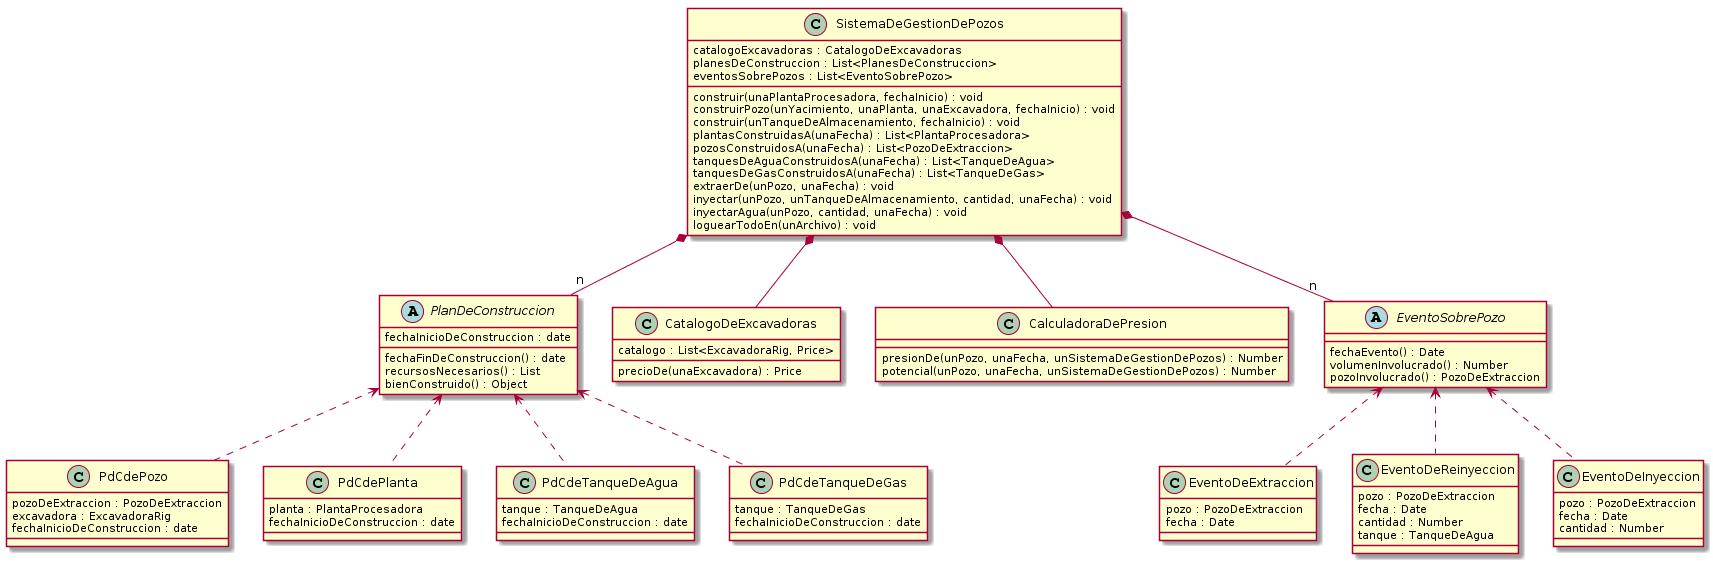
\includegraphics[angle=90,scale=0.4]{Partes/Imagenes/diagrama_alternativo1.png}
\end{figure}

\begin{figure}[H]
  \centering
  \hspace{-3.5cm}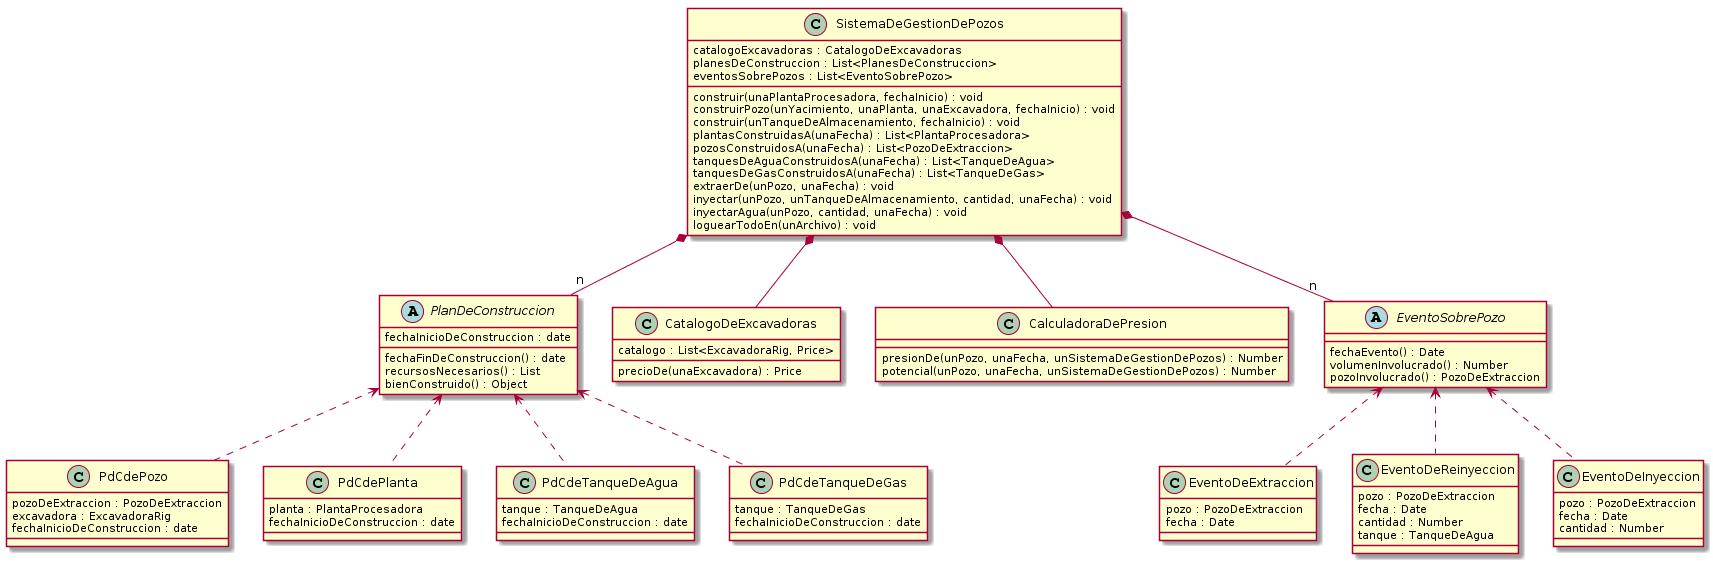
\includegraphics[angle=90,scale=0.5]{Partes/Imagenes/diagrama_alternativo1.png}
\end{figure}


\subsection{Ejecución de un criterio de construcción de pozos}

\par A continuación vamos a mostrar el diagrama de secuencias de la ejecución de un cierto criterio de construcción de pozos. Estos criterios están compuestos por tres datos importantes que pueden ser modificados:

\begin{itemize}
  \item \textbf{cantidad de pozos}: este número indica el máximo de pozos que se podrán construir. El criterio se ejcutará cada día intentando construir hasta lograr llegar a esa cantidad. Pero de igual forma, puede que el entorno y otras decisiones le impidan alcanzar este valor. Es un valor libre y a elección del usuario.
  \item \textbf{estrategia de selección de parcelas}: esto indica la forma en la cual se van a seleccionar las parcelas. Por ejemplo: en orden de profundidad, por su terreno, aleatorio, etc. Este valor se selecciona de los que el sistema permita, ya que conlleva una lógica interna.

  \item \textbf{estrategia de selección de excavadoras}: esto indica la forma en la cual se seleccionarán las excavadoras a utilizar (dentro del catálogo que se tiene) y el criterio por el cual se decidirá alquilar o no, dependiendo del momento. Al igual que el valor anterior, se selecciona dentro de opciones que el sistema brinda. Como ejemplos podemos mencionar: alquilar a demanda, alquilar como máximo 3 excavadoras, etc.
\end{itemize}

\subsubsection{Escenario}
\par En este caso nos enfocaremos en un criterio que cuenta con una cantidad máxima de 3 pozos, selecciona las parcelas con menor profunidad al reservorio y alquila excavadoras a demanda. El sistema se encuentra simulando el día 19/05/2017 y hasta el momento se construyeron 2 pozos. También contamos con items en el catálogo de excavadoras.

\subsubsection{Funcionamiento General}
\par Como vemos en el diagrama de secuencias de la figura \ref{fig:dia_sec_const_pozo_1_1}, el sistema de ejecución de criterios le envía un mensaje al criterio para que se ejecute pasándole una referencia al sistema de simulación, ya que es él quien conoce al sistema de construcción (junto con otros objetos que pueda llegar a necesitar). Este criterio es quien consulta la cantidad de pozos construidos hasta el momento y decide si se intentará construír uno nuevo. Al haber 2 pozos construidos y tener como cantidad máxima 3, le manda un mensaje a la estrategia de selección de excavadoras para que le devuelva una excavadora disponible. Como el sistema cuenta con un catálogo de excavadoras no vacío y la estrategia permite alquilar a demanda, retorna la excavadora \textit{excavadora396}. Del mismo modo, el criterio le envía un mensaje a la estrategia de selección de parcelas para que se ejecute y le retorne una parcela (en particular la \textit{parcela45-33}). Luego, consulta al sistema de simulación la fecha actual (\textit{19/05/2017}) y le envía un mensaje al sistema de construcción para que registre un plan de construcción de pozo en esa fecaha, utilizando la excavadora \textit{excavadora396} en la parcela \textit{parcela45-33}.
\par El funcionamiento interno de la estrategía de selección de parcelas se explica detalladamente a continuación en la sección \ref{sec:dia_sec_estr_selec_parc}. Mientras que el de la estrategia de selección de excavadoras se detalla en la sección \ref{sec:dia_sec_estr_selec_exc}.

\begin{landscape}
  \begin{figure}[ht]
  \centering
    \begin{sequencediagram}
      \newthread{entorno}{\shortstack{Entorno}}
      \newinst{e1}{\shortstack{elSistema\\DeEjecucion\\DeCriterios :\\SistemaDeEjecucion\\DeCriterios}}
      \newinst{e2}{\shortstack{elCriterio\\DeConstrucción\\DePozo :\\CriterioDe\\Construccion\\DePozo}}
      \newinst{e3}{\shortstack{elSimulador :\\SistemaDe\\Simulacion}}
      \newinst{e4}{\shortstack{elSistema\\DeConstrucción :\\SistemaDe\\Construccion}}
      \newinst{e5}{\shortstack{laListaDe\\PlanesActuales :\\Lista}}
      \newinst{e6}{\shortstack{laEstrategia\\DeExcavadoras :\\Estrategia\\DeAlquiler\\ADemanda}}
      \newinst{e7}{\shortstack{laEstrategia\\DeParcelas :\\Estrategia\\DeParcelas\\MenosProfundas}}

      \postlevel
      \postlevel
      \postlevel
      \begin{call}{entorno}{\shortstack{\textbf{ejecutar:}\\elCriterioDe\\Construcción\\DePozo}}{e1}{}
        \begin{call}{e1}{\shortstack{\textbf{ejecutarEn:}\\elSimulador}}{e2}{}
          \begin{call}{e2}{\shortstack{\textbf{sistemaDe}\\\textbf{Construccion}}}{e3}{\shortstack{elSistemaDe\\Construcción}}
            \postlevel
          \end{call}
          \begin{call}{e2}{\textbf{planesDeConstruccionDePozo}}{e4}{laListaDePlanesActuales}
          \end{call}
          \begin{call}{e2}{\textbf{size}}{e5}{3}
          \end{call}
          \begin{call}{e2}{\textbf{ejecutarEn:} elSimulador}{e6}{excavadora396}
          \end{call}
          \begin{call}{e2}{\textbf{ejecutarEn:} elSimulador}{e7}{parcela45-33}
          \end{call}
          \begin{call}{e2}{\textbf{fechaActual}}{e3}{19/05/2017}
          \end{call}
          \postlevel
          \postlevel
          \begin{call}{e2}{\shortstack{\textbf{comenzarConstruccionDe}\\\textbf{PozoEn:} parcela45-33\\\textbf{usando:} excavadora396\\\textbf{al:} 19/05/2017}}{e4}{}
          \end{call}
        \end{call}
      \end{call}
    \end{sequencediagram}
    \caption{Diagrama de secuencias de la ejecución de un criterio de construcción de pozo.}
    \label{fig:dia_sec_const_pozo_1_1}
  \end{figure}
\end{landscape}


\subsubsection{Funcionamiento de Estrategia de selección de parcelas}
\label{sec:dia_sec_estr_selec_parc}
\par Vamos a pasar a explicar el funcionamiento de la estrategia de selección de parcelas utilizada en el criterio antes mencionado. El diagrama de secuencia se puede ver en la figura \ref{fig:dia_sec_const_pozo_1_2}.
\par La estrategia recibe el mensaje \textit{ejecutarEn} recibiendo como parámetro el sistema de simulación (aquí instanciado como \text{elSimulador}). En primer lugar, le envía un mensaje a \textit{elSimulador} pidiéndole el sistema de gestión de parcelas, que es quien conoce las parcelas y en particular las libres (sin pozo). Luego, le envía un mensaje a este sistema de gestión de parcelas pidiéndole un listado de parcelas libres. De esta manera recibe la lista de parcelas \textit{laListaDeParcelasLibres}. Antes de continuar, le envía un mensaje a \textit{laListaDeParcelasLibre} consultándole su tamaño (cantidad de elementos). En este escenario sabemos que el sistema cuenta con parcelas libres, y en particular retorna 50. A esta lista le envía un mensaje para que se ordene, pasándole como parámetro un comparador de elementos (en este caso parcelas). Esta estrategia se basa en seleccionar las parcelas menos profundas, por lo que como comparador le envía un bloque de código que compara las parcelas por profundidad. De esta manera, la lista retorna una nueva lista de parcelas ordenada por profundidad (mencionada en el diagrama como \textit{laListaOrdenadaDeParcelasLibres}). A esta nueva lista se le envía un mensaje pidiéndole el primer elemento. La misma retorna la parcela \textit{parcela45-33}, entonces la estrategia envía un mensaje al sistema de gestión de parcelas avisándole que va a utilizar la parcela \textit{parcela45-33} (este mensaje se llama \textit{utilizarParcela} y recibe como parámetro una parcela). Para finalizar retorna la parcela \textit{parcela45-33}.

\begin{figure}[ht]
\centering
  \begin{sequencediagram}
    \newthread{entorno}{\shortstack{Entorno}}
    \newinst{e1}{\shortstack{laEstrategia\\DeParcelas\\MenosProfundas :\\EstrategiaDe\\ParcelasMenos\\Profundas}}
    \newinst{e2}{\shortstack{elSimulador :\\SistemaDe\\Simulacion}}
    \newinst{e3}{\shortstack{elSistema\\DeParcelas :\\SistemaDe\\GestiónDe\\Parcelas}}
    \newinst{e4}{\shortstack{laListaDe\\ParcelasLibres :\\Lista}}
    \newinst{e5}{\shortstack{laLista\\OrdenadaDe\\ParcelasLibres :\\Lista}}

    \postlevel
    \postlevel
    \begin{call}{entorno}{\shortstack{\textbf{ejecutarEn:}\\elSimulador}}{e1}{parcela45-33}
      \begin{call}{e1}{\shortstack{\textbf{sistemaDeGestion}\\\textbf{DeParcelas}}}{e3}{\shortstack{elSistemaDeParcelas}}
      \end{call}
      \begin{call}{e1}{\textbf{parcelasLibres}}{e3}{laListaDeParcelasLibres}
      \end{call}
      \begin{call}{e1}{\textbf{size}}{e4}{50}
      \end{call}
      \begin{call}{e1}{\textbf{ordenarPor:} unComparadorDeParcelas}{e4}{laListaOrdenadaDeParcelasLibres}
      \end{call}
      \begin{call}{e1}{\textbf{first}}{e5}{parcela45-33}
      \end{call}
      \begin{call}{e1}{\textbf{utilizarParcela:} parcela45-33}{e3}{}
      \end{call}
    \end{call}
  \end{sequencediagram}
  \caption{Diagrama de secuencias de la ejecución de la estrategia de selección de pozos menos profundos.}
  \label{fig:dia_sec_const_pozo_1_2}
\end{figure}

\subsubsection{Funcionamiento de Estrategia de selección de excavadoras}
\label{sec:dia_sec_estr_selec_exc}
\par La figura \ref{fig:dia_sec_const_pozo_1_3} muestra el diagrama de secuencias de la ejecución de la estrategia de selección de excavadoras a demanda. Esta estrategia simplemente busca en el catálogo de excavadoras una y la alquila, sin tener en cuenta el precio o las excavadoras previamente alquiladas con tiempo ocioso.

\par La estrategia recibe el mensaje \textit{ejecutarEn}, junto con un sistema de simulación como parámetro (mencionado como \textit{elSimulador}). Le pide a \textit{elSimulador} el sistema de gestión de excavadoras (quien conoce el catálogo y puede alquilar excavadoras). Luego le envía un mensaje a este sistema consultando consultándole las excavadoras disponibles (items del catálogo de excavadoras). De esta manera recibe una lista de excavadoras (en el diagrama \textit{laListaDeExcavadorasDisponibles}), a la cual le consulta su tamaño (cantidad de excavadoras). En el escenario actual, sabemos que el sistema cuenta con un catálogo con excavadoras (en particular 3). Entonces, a \textit{laListaDeExcavadorasDisponibles} se le envía un mensaje pidiendo el primer elemento de la lista, la cual retorna \textit{itemExcavadora10}. A este item del catálogo se le envía un mensaje consultado su modelo (\textit{modeloDeExcavadora}), el cual retorna \textit{E-123}. De esta manera ya se tiene seleccionado un modelo de excavadora del catálogo, y como la estrategia se basa en alquilar a demanda, le envía al sistema de gestión de excavadoras el mensaje \textit{alquilarExcavadoraDeModelo} pasándole como parámetro el modelo \textit{E-123}. Al recibir este mensaje, el sistema de gestión de excavadoras crea una nueva excavadora (del modelo \textit{E-123}) y la retorna. La estrategia recibe a la excavadora recién alquilada \textit{excavadora396} y la retorna.
\begin{figure}[ht]
\centering
  \begin{sequencediagram}
    \newthread{entorno}{\shortstack{Entorno}}
    \newinst{e1}{\shortstack{laEstrategiaDe\\AlquilerADemanda :\\EstrategiaDeAlquiler\\ADemanda}}
    \newinst{e2}{\shortstack{elSimulador :\\SistemaDe\\Simulacion}}
    \newinst{e3}{\shortstack{elSistema\\DeExcavadras :\\SistemaDe\\GestiónDe\\Excavadoras}}
    \newinst{e4}{\shortstack{laListaDe\\Excavadoras\\Disponibles :\\Lista}}
    \newinst{e5}{\shortstack{itemExcavadora10 :\\ItemDeAlquiler}}

    \postlevel
    \begin{call}{entorno}{\shortstack{\textbf{ejecutarEn:}\\elSimulador}}{e1}{excavadora396}
      \begin{call}{e1}{\shortstack{\textbf{sistemaDeGestion}\\\textbf{DeExcavadoras}}}{e3}{\shortstack{elSistemaDeExcavadoras}}
      \end{call}
      \begin{call}{e1}{\textbf{excavadorasDisponibles}}{e3}{\shortstack{laListaDeExcavadoras\\Disponibles}}
        \postlevel
      \end{call}
      \begin{call}{e1}{\textbf{size}}{e4}{3}
      \end{call}
      \begin{call}{e1}{\textbf{first}}{e4}{itemExcavadora10}
      \end{call}
      \begin{call}{e1}{\textbf{modeloDeExcavadora}}{e5}{E-123}
      \end{call}
      \postlevel
      \begin{call}{e1}{\shortstack{\textbf{alquilarExcavadoraDe}\\\textbf{Modelo:} E-123}}{e3}{excavadora396}
      \end{call}
    \end{call}
  \end{sequencediagram}
  \caption{Diagrama de secuencias de la ejecución de la estrategia de selección de excavadora alquilando a demanda.}
  \label{fig:dia_sec_const_pozo_1_3}
\end{figure}


\subsection{Ejecución de un criterio de construcción de plantas}

\par Mostraremos a continuación el diagrama de secuencias que muestra la ejecución de un criterio de construcción de plantas procesadoras. Este tipo de criterios se crean a partir de una estrategia de construcción de plantas, la cual consta de dos partes importantes:

\begin{itemize}
  \item \textbf{estrategia de cantidad de plantas procesadoras}: esta puede ser de dos tipos: limitada o ilimitada. Las de tipo ilimitada permiten construir infinitas plantas procesadoras, mientras que las limitadas se crean con un número que indica la cantidad máxima de plantas procesadoras que se podrán construir a lo largo de toda la simulación.
  \item \textbf{estrategia de selección de plantas procesadoras}: la cual se encarga de seleccionar del catálogo, que se encuentra precargado, las plantas que se van a construir. Por ejemplo: se pueden elegir las mas baratas, o las que tengan mayor volumen de procesamiento diario, etc.
\end{itemize}

\subsubsection{Escenario}
\par En este caso nos encontramos con un criterio compuesto por una estrategia de construcción de plantas que construye todas las plantas procesadoras que pueda el primer día de simulación, mientras que el resto de los días no construye mas. Para controlar la cantidad de plantas procesadoras a construir se utiliza una estrategia que limita la cantidad máxima a 1. La estrategia de selección de plantas procesadoras utilizada selecciona del catálogo las plantas ordenada por capacidad de procesamiento diario, de mayor a menor.
\par Al momento de recibirse este mensaje, el sistema de simulación recibido como parámetro se encuentra en el primer día de simulación, con fecha 10/05/2017. El mismo cuenta con un pozo de extracción construído y sin ninguna planta procesadora, ya que es el primer día y los criterios se ejecutan una única vez por día.

\subsubsection{Funcionamiento General}
\par Bajo el escenario mencionado, sabemos que queda una planta procesadora por construir y hay un pozo de extracción que no está conectado a ninguna planta procesadora. Veremos a continuación como el funcionamiento del criterio lleva a que se construya una planta procesadora y se la contecte a el pozo.
\par Para el criterio de construcción de plantas procesadoras que estamos mostrando en el escenario elegido, podemos dividir el funcionamiento en dos partes:
\begin{itemize}
  \item Construcción de plantas: aquí se consulta a la estrategia de cantidad de plantas y luego se construyen las plantas que se requieran. Esta parte se realiza solo el primer día de ejecución.
  \item Conexión de plantas a pozos libres: aquí se verifica que todos los pozos del sistema se encuentren conectados a una planta procesadora. Esto se realiza todos los días. Si se encuentra un pozo libre se lo conecta a la planta procesadora con menor cantidad de conexiones. Esto es una determinación tomada para simplificar el funcionamiento general en una primer versión del sistema.
\end{itemize}
\par Con el panorama general ya planteado, pasaremos entonces a explicar el diagrama de secuencia de la figura \ref{fig:dia_sec_const_planta_1_1}, que muestra el funcionamiento del criterio de construcción de plantas al recibir el mensaje de ejecución.
\par Llega el mensaje \textit{ejecutarEn}, junto con \textit{elSimulador} como parámetro al criterio de construccion de edificación \textit{elCriterioDeConstrucciónDePlantas}. Este criterio, lo único que hace es redirigirlo a su estrategia de construcción de plantas (\textit{laEstrategiaDeConstrucciónDePlantas}) con un mensaje de igual nombre. La estrategia recibe este mensaje y lo primero que hace es consultarse a si mismo si se encuentra en el primer día de simulación, esto para diferenciar qué partes (de las dos antes mencionadas) debe realizar. Recibe \textit{Verdadero}, por lo cual va a realizar ambas partes.
\par Primero la parte de construcción de plantas. Para esto le envía un mensaje a \textit{laEstrategiaDeCantidadDePlantas} para consultarle si debe intentar construir una planta procesadora. En caso de que ya se haya llegado al límite, la estrategia le responderá \textit{Verdadero}. Pero sobre el escenario planteado queda una planta procesadora por construir, por lo que responde \textit{Falso}. Por esto, se envía un mensaje a si mismo: \textit{nuevaPlantaEn}, pasándose \textit{elSimulador} como parámetro. El funcionamiento de este mensaje se explica detalladamente en la sección \ref{sec:dia_sec_estr_nuevaplanta}. Al retornar, vuelve a consultar a la estrategia \textit{laEstrategiaDeCantidadDePlantas} para saber si debe volver a intentar construir una nueva planta procesadora. En este caso, responde \textit{Verdadero} (ya que se alcanzó el máximo), lo que implica que no se deben construir mas.
\par A continuación, procede a realizar la parte dos: conexión de plantas a pozos libre. La estrategia \textit{laEstrategiaDeConstrucciónDePlantas} se envía un mensaje a si mismo consultando si hay pozos libres en el sistema (por medio del mensaje \textit{hayUnPozoLibreEn}). En el escenario planteado, se retorna \textit{Verdadero} y en consecuencia se envía otro mensaje pidiendo un pozo libre (sabiendo que hay uno). Este mensaje es \textit{pozoLibreEn}, y envía el sistema de simulación como parámetro para poder averiguar lo necesario. De este mensaje se retorna el pozo \textit{elPozo1}. Luego, la estrategia se consulta a si mismo por la planta menos usada, por medio del mensaje \textit{plantaMenosUsada}. Este mensaje retorna la única planta y por lo tanto la que cuenta con menor cantidad de pozos conectados: \textit{laPlantaProc1}. Para finalizar, le pide al sistema de simulación el sistema de construcción por medio del mensaje \textit{elSistemaDeConstrucción} y le envía el mensaje \textit{conectar: elPozo1 a: laPlantaProc1}.

\begin{figure}[ht]
\centering
  \begin{sequencediagram}
    \newinst{e1}{\shortstack{elCriterioDe\\Construcción\\DePlantas :\\CriterioDe\\Construccion\\DeEdificacion}}
    \newinst{e2}{\shortstack{laEstrategia\\DeConstrucción\\DePlantas :\\EstrategiaDe\\ConstruccionDe\\PlantaAlInicio}}
    \newinst{e3}{\shortstack{laEstrategia\\DeCantidad\\DePlantas :\\EstrategiaDe\\PlantasLimitadas}}
    \newinst{e4}{\shortstack{elSimulador :\\SistemaDe\\Simulacion}}
    \newinst{e5}{\shortstack{elSistemaDe\\Construcción :\\SistemaDe\\Construccion}}

    \postlevel
    \postlevel
    \begin{call}{}{\shortstack{\textbf{ejecutarEn:}\\elSimulador}}{e1}{}
      \begin{call}{e1}{\shortstack{\textbf{ejecutarEn:}\\elSimulador}}{e2}{}
        \begin{callself}{e2}{\textbf{esElPrimerDiaEn:} elSimulador}{Verdadero}
        \end{callself}

        \postlevel
        \begin{call}{e2}{\shortstack{\textbf{ejecutarEn:}\\elSimulador}}{e3}{Falso}
        \end{call}
        \begin{callself}{e2}{\textbf{nuevaPlantaEn:} elSimulador}{}
        \end{callself}
        \postlevel
        \begin{call}{e2}{\shortstack{\textbf{ejecutarEn:}\\elSimulador}}{e3}{Verdadero}
        \end{call}

        \begin{callself}{e2}{\textbf{hayUnPozoLibreEn:} elSimulador}{Verdadero}
        \end{callself}
        \begin{callself}{e2}{\textbf{pozoLibreEn:} elSimulador}{elPozo1}
        \end{callself}
        \begin{callself}{e2}{\textbf{plantaMenosUsada}}{laPlantaProc1}
        \end{callself}
        \begin{call}{e2}{\textbf{sistemaDeConstruccion}}{e4}{elSistemaDeConstrucción}
        \end{call}
        \begin{call}{e2}{\textbf{conectar:} elPozo1 \textbf{a:} laPlantaProc1}{e5}{}
        \end{call}

      \end{call}
    \end{call}
  \end{sequencediagram}
  \caption{Diagrama de secuencias de la ejecución de un criterio de construcción de plantas procesadoras todas el primer día.}
  \label{fig:dia_sec_const_planta_1_1}
\end{figure}

\subsubsection{Funcionamiento de Estrategia de construcción de plantas ante el mensaje nuevaPlantaEn}
\label{sec:dia_sec_estr_nuevaplanta}
\par El diagrama de secuencia que se explicará a continuación corresponde con la figura \ref{fig:dia_sec_const_planta_1_2}.
\par La estrategia recibe el mensaje \textit{nuevaPlantaEn} junto con \textit{elSimulador} (un sistema de simulación). Lo primero que hace es consultar la fecha actual de simulación. Para esto envía el mensaje \textit{fechaDeSimulacion} a \textit{elSimulador}, el cual retorna \textit{10/05/2017}. Luego le envía un mensaje a la estrategia de selección de de plantas que conoce para que se ejecute y le retorne un item del catálogo de plantas procesadoras. En este caso, retorna el item \textit{itemPlanta3}, debido a que es la planta con mayor nivel de procesamiento diario. Tras seleccionar un item del catálogo, le envía el mensaje \textit{modeloDeItem} para obtener el modelo de planta. En el escenario planteado se retorna el modelo \textit{P-A2}. También le envía el mensaje \textit{plazoDeConstruccion}, el cual retorna \textit{20} (cantidad de días necesarios para la construcción de una planta de este modelo). Luego, le envía el mensaje \textit{addDays: 20} a la fecha \textit{10/05/2017} (que antes había obtenido), el cual retorna una nueva fecha \textit{30/05/2017}. Finalmente crea una nueva instancia de una planta procesadora pasándole \textit{P-A2} (el modelo antes obtenido), el cual retorna \textit{laPlantaProc1} y le envía un mensaje al sistema de construcción para que cree el plan de construcción de planta procesadora: \textit{comenzarConstruccionDePlantaProcesadora: laPlantaProc1 arrancandoEl: 10/05/2017 yFinalizando: 30/05/2017}.

\begin{landscape}
  \begin{figure}[ht]
  \centering
    \begin{sequencediagram}
      \newinst{e1}{\shortstack{laEstrategia\\DeConstruccion\\DePlantas :\\EstrategiaDe\\ConstruccionDe\\PlantaAlInicio}}
      \newinst{e2}{\shortstack{elSimulador :\\SistemaDe\\Simulacion}}
      \newinst{e3}{\shortstack{10/05/2017 :\\Fecha}}
      \newinst{e4}{\shortstack{laEstrategia\\DeSelección\\DePlantas :\\EstrategiaDe\\PlantaCon\\MayorCapacidad}}
      \newinst{e5}{\shortstack{itemPlanta3 :\\ItemDeConstruccion}}
      \newinst{e6}{PlantaProcesadora}
      \newinst{e7}{\shortstack{elSistemaDe\\Construcción :\\SistemaDe\\Construccion}}

      \postlevel
      \postlevel
      \begin{call}{}{\shortstack{\textbf{nuevaPlantaEn:}\\elSimulador}}{e1}{}
        \begin{call}{e1}{\textbf{fechaDeSimulacion}}{e2}{10/05/2017}
        \end{call}
        \begin{call}{e1}{\textbf{ejecutarEn:} elSimulador}{e4}{itemPlanta3}
        \end{call}
        \begin{call}{e1}{\textbf{modeloDeItem}}{e5}{P-A2}
        \end{call}
        \begin{call}{e1}{\textbf{plazoDeConstruccion}}{e5}{20}
        \end{call}
        \begin{call}{e1}{\textbf{addDays:} 20}{e3}{30/05/2017}
        \end{call}
        \begin{call}{e1}{\textbf{new deModelo:} P-A2}{e6}{laPlantaProc1}
        \end{call}
        \postlevel
        \begin{call}{e1}{\shortstack{\textbf{comenzarConstruccionDePlantaProcesadora:} laPlantaProc1 \\ \textbf{arrancandoEl:} 10/05/2017 \textbf{yFinalizando:} 30/05/2017}}{e7}{}
        \end{call}
      \end{call}
    \end{sequencediagram}
    \caption{Diagrama de secuencias de la construcción de una nueva planta por medio de una estrategia de construcción de plantas procesadoras todas el primer día.}
    \label{fig:dia_sec_const_planta_1_2}
  \end{figure}
\end{landscape}


\subsection{Ejecución de un criterio de parada}

\par A continuación vamos a mostrar el diagrama de secuencias de la ejecución del criterio de parada que es el que determina la finalización de la simulación. Va a estar compuesto por una estrategia de parada y un parámetro representativo de la estrategia (por ejemplo, una estrategia de parada podría ser "hasta que el yacimiento tenga cierto nivel de presión de los pozos" y el parámetro representativo sería ese valor de presión). Este criterio se ejecutará cada día (luego de haber ejecutado los criterios de construcción, de extracción, etc) de manera de indicarle al sistema de ejecución de criterios si debe finalizar o no la simulación (devuelve true en dicho caso). A continuación describiremos el diagrama de secuencia correspondiente a este criterio.


\subsubsection{Escenario}
\par En este caso nos enfocaremos en un criterio que determina la finalizaci�n de la simulación un vez que hayan pasado 150 días. El sistema se encuentra simulando el día 10/12/2017 y la fecha de inicio fue el 01/09/2017.

\subsubsection{Funcionamiento General}
\par Como vemos en el diagrama de secuencias de la figura \ref{fig:dia_sec_parada_1_1}, el sistema de ejecución de criterios le envía un mensaje al criterio para que se ejecute pasándole una referencia al sistema de simulación, ya que es él quien conoce los objetos fechaDeSimulación y fechaDeInicio. Este criterio le envía el mensaje ejecutar a la estrategia elegida por el usuario, que en este caso es de tipo EstrategiaDeParadaPorCantidadDeDias. Luego, la estrategia le consulta al Simulador qué fecha está simulando y cuál es la fecha de inicio. Internamente hace la resta entre las dos fechas, y le responde false a elCriterioDeParada una vez que el resultado fue menor a 150 días.

\begin{landscape}
  \begin{figure}[ht]
  \centering
    \begin{sequencediagram}
      \newinst{e1}{\shortstack{elSistema\\DeEjecucion\\DeCriterios :\\SistemaDeEjecucion\\DeCriterios}}
      \newinst{e2}{\shortstack{elCriterio\\DeParada :\\CriterioDe\\Parada}}
      \newinst{e3}{\shortstack{laEstrategia\\DeParada :\\Estrategia\\DeParada\\PorCantidad\\DeDias}}
      \newinst{e4}{\shortstack{elSimulador :\\SistemaDe\\Simulacion}}

      \postlevel
      \postlevel
      \postlevel
      \begin{call}{}{\shortstack{\textbf{ejecutar:}\\elCriterioDe\\Parada}}{e1}{true}
        \begin{call}{e1}{\shortstack{\textbf{ejecutarEn:}\\elSimulador}}{e2}{true}
          \begin{call}{e2}{\shortstack{\textbf{ejecutarEn:}\\elSimulador}}{e3}{true}
            \begin{call}{e3}{\shortstack{\texbf{fechaDe\\Simulacion}}}{e4}{10/12/2017}
            \postlevel
            \end{call}
            \postlevel
            \begin{call}{e3}{\shortstack{\texbf{fechaDe\\Inicio}}}{e4}{10/12/2017}
            
            \postlevel
            \end{call}
          \end{call}
        \end{call}
      \end{call}
    \end{sequencediagram}
    \caption{Diagrama de secuencias de la ejecuci�n de un criterio de parada.}
    \label{fig:dia_sec_parada_1_1}
  \end{figure}
\end{landscape}


\subsection{Aclaraciones / Futuras mejoras}

\par Acá la idea sería poner cosas que "supusimos" o tomamos como válidas. Explicar por qué.
\par También poner cosas que dejamos "duras" y que van a ser futuras mejoras.


\begin{itemize}
  \item Por ejemplo cuando creas de entrada mas plantas q pozos, te pueden llegar a quedar plantas libres.. Entonces al crear un nuevo pozo, tenes q elegir a que planta lo conectas. Por ahora solo se está eligiendo "la menos usada". Esto en un futuro debería ser una estrategia y que se pueda modificar.
\end{itemize}



\end{document}
